\section{Implementation \& Systems Mechanics}
\label{sec:implementation}

The formal properties and empirical behavior of state virtualization and predictive residency depend directly on runtime mechanics. In this section, we detail the concrete implementation of the ModelVM execution engine. We describe the runtime control loop, the serialization and delta-tracking mechanics of the Cognitive State Packet, the memory accounting and eviction dynamics of the Model Pager, the lookahead forecasting engine of the Working Set Predictor, and the physical telemetry instrumentation layer that records hardware ground truth.

\subsection{The Runtime Control Loop}
\label{sec:runtime_loop}

The ModelVM runtime is orchestrated by the \textbf{Cognitive Kernel} (\texttt{CognitiveKernel}), which functions as a kernel-inspired supervisory runtime component for heterogeneous language model execution. Rather than treating model invocation as an ad-hoc chain of stateless remote procedure calls, the kernel coordinates execution through a deterministic four-phase state machine: \textit{Planning}, \textit{Residency Allocation}, \textit{Execution \& AST Verification}, and \textit{State Persistence \& Escalation}.

\begin{figure*}[t]
\centering
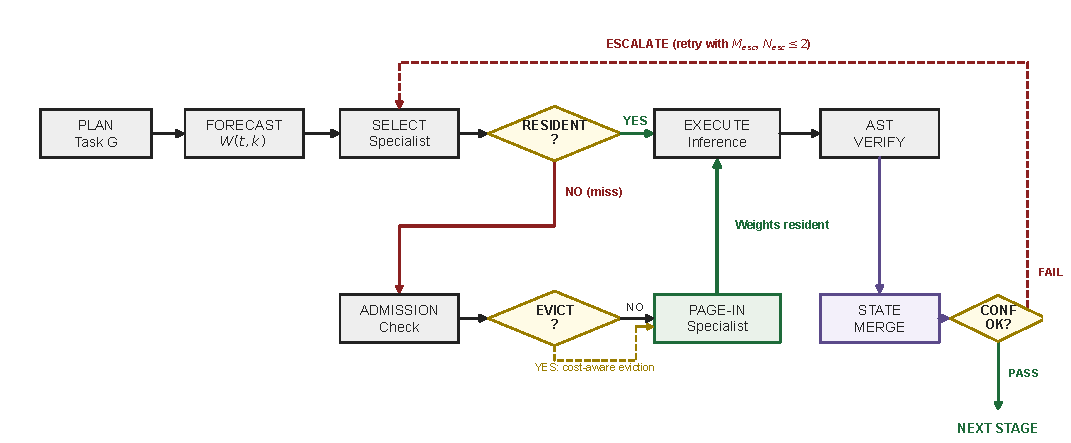
\includegraphics[width=\textwidth]{fig4_control_path.pdf}
\caption{ModelVM End-to-End Architectural Control Path (Class B full-width). The Cognitive Kernel orchestrates procedural task decomposition, working-set demand forecasting $W(t, k)$, multi-objective scheduling, memory-budgeted weight paging with eviction shielding, specialist execution, non-circular AST verification, and diversity-discounted state merging with bounded escalation.}
\label{fig:control_path}
\end{figure*}

Formally, the runtime transition function at pipeline stage $t \in \{0, \dots, N-1\}$ maps the current state packet $\mathcal{S}_t$, the stage task specification $s_t$, and the active resident model set $\mathcal{R}_t$ to the successor state $\mathcal{S}_{t+1}$:
\begin{equation}
\begin{aligned}
(\mathcal{S}_t, s_t, \mathcal{R}_t) &\xrightarrow{\text{Forecast}} (W_t, M_t) \xrightarrow{\text{PageIn}} \mathcal{R}_{t+1} \\
&\xrightarrow{\text{Exec}} \Delta \mathcal{S}_t \xrightarrow{\text{Merge}} \mathcal{S}_{t+1}
\end{aligned}
\label{eq:state_transition_machine}
\end{equation}
where $W_t = W(t, k)$ is the predicted future working set, $M_t$ is the selected executing specialist, and $\Delta \mathcal{S}_t$ is the candidate state delta generated by the model.

\paragraph{1. Planning Phase.}
Execution begins with the \texttt{TaskDecomposer}. Given an overarching user objective $G$, the decomposer produces a directed acyclic graph (DAG) of stage plans $G_{\text{plan}} = (S, E)$, where each stage $s_t \in S$ encapsulates a title, an instruction description, and an explicit target capability annotation $C(s_t) \in \mathcal{C}$ (e.g., \textsc{Research}, \textsc{Mathematics}, \textsc{Coding}, \textsc{Physics}, \textsc{Synthesis}). The root state packet $\mathcal{S}_0$ is initialized with objective $G$ and an empty accumulation schema.

\paragraph{2. Residency Phase.}
Before executing stage $s_t$, the kernel queries the \texttt{CognitiveWorkingSetPredictor} to project future capability demand across lookahead horizon $k$, returning $W(t, k)$. Next, the \texttt{CognitiveScheduler} evaluates all eligible models in catalog $\mathcal{M}$ using a multi-objective scoring function that incorporates capability fit, memory footprint, load latency, energy consumption, eviction penalties, and working-set alignment. The winning model $M_t$ is dispatched to the \texttt{ModelPager}. The pager checks whether $M_t \in \mathcal{R}_t$. If $M_t$ is resident, a cache hit is recorded with zero page-in latency. If $M_t$ is not resident, the pager computes the memory deficit $\Delta_{\text{mem}} = \text{RAM}(M_t) - \text{RAM}_{\text{free}}$ and executes cost-aware evictions until the hard memory budget invariant is satisfied:
\begin{equation}
\sum_{m_i \in \mathcal{R}_t} \text{RAM}(m_i) \le \mathcal{B}_{\text{RAM}}
\end{equation}
Once memory space is reserved, weights are staged into active memory. If free memory remains and exceeds an explicit safety headroom buffer of 1.0\,GB, the predictor evaluates the prefetch return-on-investment (ROI) and opportunistically stages an upcoming model $M_{t+1}$ before stage execution.

\paragraph{3. Execution \& Verification Phase.}
With $M_t$ resident, the kernel serializes the current state packet $\mathcal{S}_t$ into a structured Markdown prompt context via \texttt{to\_prompt\_context()} and dispatches it to the model backend (\texttt{ModelBackend}). The specialist generates its domain response within a strict token budget. The raw generation is parsed by \texttt{extract\_from\_text()} into a candidate state delta $\Delta \mathcal{S}_t$. Crucially, numerical and algebraic claims within $\Delta \mathcal{S}_t$ are immediately intercepted by an independent Abstract Syntax Tree verifier (\texttt{ArithmeticVerifier}). The verifier parses the declared mathematical expressions and evaluates them against computed numerical results. Calculations that satisfy numerical equivalence within relative tolerance $\epsilon = 10^{-3}$ are tagged with \texttt{verified=True}; failed or unparsable expressions remain unverified. Language models are never permitted to self-grade their own arithmetic outputs.

\paragraph{4. State Persistence \& Escalation Phase.}
The verified delta $\Delta \mathcal{S}_t$ is merged into the global state packet using monotonic accumulation mechanics: $\mathcal{S}_{t+1} = \mathcal{S}_t.\text{merge\_update}(\Delta \mathcal{S}_t)$. Once merged, the \texttt{ConfidenceController} evaluates the composite confidence score of stage $t$. If confidence falls below threshold $\tau_{\text{conf}} = 0.70$ or if open questions remain unresolved, the controller triggers an escalation loop. To prevent infinite cycles, escalation is governed by strict loop protection:
\begin{itemize}
    \item Maximum escalations per stage are bounded at $N_{\text{esc}} \le 2$.
    \item A candidate escalation model $M_{\text{esc}}$ must provide a strictly higher capability-quality product than the current model: $(F_{\text{cap}}(M_{\text{esc}}) \cdot Q(M_{\text{esc}})) - (F_{\text{cap}}(M_t) \cdot Q(M_t)) \ge \epsilon_{\text{esc}}$ with $\epsilon_{\text{esc}} = 0.02$.
    \item $M_{\text{esc}}$ must physically fit within the runtime memory envelope $\mathcal{B}_{\text{RAM}}$.
\end{itemize}
If a qualifying escalation model exists, the kernel pages in $M_{\text{esc}}$, re-executes the stage with explicit refinement instructions, and merges the refined delta. Once confidence criteria are met or the escalation ceiling is reached, the stage execution telemetry is broadcast to listeners and recorded to persistent disk storage.

The full control sequence is formalized in Algorithm~\ref{alg:control_loop}.

\begin{algorithm}[htbp]
\caption{ModelVM Runtime Control Loop}
\label{alg:control_loop}
\footnotesize
\begin{algorithmic}[1]
\Require Task goal $G$, Model catalog $\mathcal{M}$, Memory budget $\mathcal{B}_{\text{RAM}}$, Lookahead horizon $k$
\Ensure Final structured state packet $\mathcal{S}_N$, Execution summary $\mathcal{T}$
\State $\mathcal{S}_0 \gets \text{InitStatePacket}(G)$
\State $S \gets \text{DecomposeTask}(G)$ \Comment{Directed stage plan $S = [s_0, \dots, s_{N-1}]$}
\State $\mathcal{R}_0 \gets \emptyset$, $\quad \text{PeakMem} \gets 0.0$
\For{$t \gets 0$ \textbf{to} $N-1$}
    \State $C_t \gets s_t.\text{capability}$
    \State $W_t \gets \text{PredictWorkingSet}(S, t, k, \mathcal{M})$ \Comment{Lookahead model IDs}
    \State $M_t \gets \text{ScheduleModel}(C_t, W_t, \mathcal{R}_t, \mathcal{M}, \mathcal{B}_{\text{RAM}})$
    \State $\mathcal{E}_{\text{page}} \gets \text{PageIn}(M_t, \mathcal{R}_t, \mathcal{B}_{\text{RAM}}, W_t)$ \Comment{Evicts if needed}
    \State $\mathcal{R}_{t+1} \gets \mathcal{R}_t \cup \{M_t\} \setminus \text{EvictedModels}$
    \State $\text{PeakMem} \gets \max(\text{PeakMem}, \sum_{m \in \mathcal{R}_{t+1}} \text{RAM}(m))$
    \If{$U_{\text{prefetch}}(M_{\text{next}}) > 0 \land (\text{RAM}_{\text{free}} - \text{RAM}(M_{\text{next}}) \ge 1.0\,\text{GB})$}
        \State $\text{PrefetchModel}(M_{\text{next}}, W_t)$ \Comment{Admitted via positive ROI \& headroom}
    \EndIf
    \State $\Pi_t \gets \text{SerializeToPrompt}(\mathcal{S}_t, s_t)$
    \State $\mathbf{y}_t \gets \text{ExecuteInference}(M_t, \Pi_t)$ \Comment{Specialist inference}
    \State $\Delta \mathcal{S}_t \gets \text{ExtractStateDelta}(G, \mathbf{y}_t, t)$
    \State $\Delta \mathcal{S}_t \gets \text{VerifyCalculations}(\Delta \mathcal{S}_t)$ \Comment{Independent AST verifier}
    \State $\mathcal{S}_{t+1} \gets \mathcal{S}_t.\text{merge\_update}(\Delta \mathcal{S}_t)$
    \State $\kappa \gets \text{EvaluateConfidence}(\mathcal{S}_{t+1}, M_t, C_t)$
    \State $n_{\text{esc}} \gets 0$
    \While{$\kappa.\text{escalation\_needed} \textbf{ and } n_{\text{esc}} < 2$}
        \State $M_{\text{esc}} \gets \text{SelectEscCandidate}(C_t, M_t, \mathcal{M}, \mathcal{B}_{\text{RAM}})$
        \If{$M_{\text{esc}} = \text{None} \textbf{ or } M_{\text{esc}} = M_t$} \textbf{break} \EndIf
        \State $\text{PageIn}(M_{\text{esc}}, \mathcal{R}_{t+1}, \mathcal{B}_{\text{RAM}}, W_t)$
        \State $\mathbf{y}_{\text{esc}} \gets \text{ExecuteInference}(M_{\text{esc}}, \Pi_t, \kappa.\text{reason})$
        \State $\Delta \mathcal{S}_{\text{esc}} \gets \text{ExtractStateDelta}(G, \mathbf{y}_{\text{esc}}, t)$
        \State $\Delta \mathcal{S}_{\text{esc}} \gets \text{VerifyCalculations}(\Delta \mathcal{S}_{\text{esc}})$
        \State $\mathcal{S}_{t+1} \gets \mathcal{S}_{t+1}.\text{merge\_update}(\Delta \mathcal{S}_{\text{esc}})$
        \State $M_t \gets M_{\text{esc}}$, $\quad n_{\text{esc}} \gets n_{\text{esc}} + 1$
        \State $\kappa \gets \text{EvaluateConfidence}(\mathcal{S}_{t+1}, M_t, C_t)$
    \EndWhile
    \State $\text{RecordStageTelemetry}(t, M_t, \mathcal{E}_{\text{page}}, \kappa, \mathcal{S}_{t+1})$
\EndFor
\State \Return $\mathcal{S}_N, \text{BuildSummaryReport}()$
\end{algorithmic}
\end{algorithm}

\subsection{CSP Schema Serialization \& Delta Tracking}
\label{sec:csp_serialization}

The \textbf{Cognitive State Packet (CSP)} virtualizes task memory by decoupling problem semantics from tokenizer representations and latent activation geometries. In the ModelVM codebase, CSP is implemented as a strongly typed data structure (\texttt{CognitiveStatePacket}) defined via Pydantic schema validation.

\paragraph{Schema Formalism.}
The state packet $\mathcal{S}_t$ at stage $t$ is defined as the 9-tuple:
\begin{equation}
\mathcal{S}_t = \langle G, F_t, C_t, E_t, A_t, U_t, D_t, Q_t, O_t \rangle
\end{equation}
where:
\begin{itemize}
    \item $G \in \Sigma^*$ is the immutable user goal string.
    \item $F_t = \{f_1, \dots, f_m\} \subset \Sigma^*$ is the deduplicated set of verified factual statements accumulated across stages.
    \item $C_t = \{c_1, \dots, c_p\}$ is the sequence of structured calculation records (\texttt{CalculationItem}). Each item encapsulates:
    \begin{equation}
    c = \langle \text{expr}, \text{result}, \text{unit}, \text{verified}, \text{method} \rangle
    \end{equation}
    where $\text{verified} \in \{\text{True}, \text{False}\}$ and $\text{method} \in \{\text{arithmetic}, \text{symbolic}, \text{None}\}$.
    \item $E_t = \{e_1, \dots, e_q\}$ is the set of empirical evidence items (\texttt{EvidenceItem}). Each item encapsulates:
    \begin{equation}
    e = \langle \text{claim}, \text{source}, \text{conf}, \text{time}, \text{model\_id} \rangle
    \end{equation}
    with confidence scalar $c \in [0.0, 1.0]$ and explicit provenance tracking.
    \item $A_t, U_t, D_t, Q_t \subset \Sigma^*$ represent working assumptions, known uncertainties, architectural decisions, and unresolved open questions, respectively.
    \item $O_t = \{k_i \mapsto v_i\}$ is the concrete artifact dictionary mapping unique semantic keys to generated digital deliverables (e.g., Python scripts, numerical matrices, simulation outputs, LaTeX tables).
    \item In addition, $\mathcal{S}_t$ maintains a persistent execution audit log $H_t = [h_0, \dots, h_{t-1}]$ of \texttt{StageTrace} records capturing model IDs, execution latencies, and timestamps.
\end{itemize}

\paragraph{Prompt Context Serialization.}
To pass state across heterogeneous models with mutually incompatible tokenizers, $\mathcal{S}_t$ implements \texttt{to\_prompt\_context()}. This method serializes the structured state into a clean, markdown-delimited prompt context. Factual records, verified calculations, evidence items, and prior decisions are formatted into distinct semantic blocks. Calculations explicitly indicate their verification status (e.g., \texttt{[VERIFIED: arithmetic]} versus \texttt{[UNVERIFIED]}). Artifacts containing multiline code or tables are fenced with syntax identifiers. This prompt serialization ensures that downstream specialist models receive an unambiguous, human-readable summary of prior state without experiencing raw conversational noise.

\paragraph{Epistemic Evidence Aggregation.}
When multiple models generate evidence supporting identical or related claims, ModelVM accumulates confidence through a diversity-discounted heuristic:
\begin{equation}
p_{\text{merged}} = \begin{cases}
\max(c_1, c_2), & \text{if } s_1 \approx s_2 \\[3pt]
\min\left(0.99, \;\max(c_1, c_2, \, c_{\text{indep}})\right), & \text{if } s_1 \not\approx s_2
\end{cases}
\label{eq:evidence_aggregation}
\end{equation}
where $c_{\text{indep}} = 1 - (1 - c_1)(1 - c_2)^{w_{\text{div}}}$ and $w_{\text{div}} = 0.65$ is the epistemic diversity discount factor. Systems claims require empirical honesty: language models share vast pretraining corpora (e.g., Common Crawl, Wikipedia, GitHub) and cannot be modeled as independent statistical observers. When two distinct specialist models produce matching claims, the exponent $w_{\text{div}} = 0.65$ dampens confidence growth, preventing unjustified certainty inflation. If claims originate from identical or overlapping sources ($s_1 \approx s_2$), the maximum rule is applied, preventing self-reinforcing echo loops.

\paragraph{Artifact Conflict Versioning.}
Concurrent or multi-stage pipelines frequently generate conflicting deliverables under identical variable names. The method \texttt{merge\_artifacts()} detects key collisions. If incoming artifact $k \in \Delta \mathcal{S}_t$ shares a key with existing artifact $k \in \mathcal{S}_t$ but contains divergent content ($v_{\text{new}} \neq v_{\text{old}}$), ModelVM preserves the original and assigns the update to a versioned key $k\text{\_v}N$ ($N \ge 1$). Furthermore, the system flags the collision by setting $k\text{\_CONFLICT} = \text{True}$. This non-destructive versioning prevents silent data overwrites during specialist transitions.

\paragraph{Monotonic State Accumulation.}
The method \texttt{merge\_update()} accumulates knowledge monotonically:
\begin{itemize}
    \item \textbf{Facts:} New facts are appended subject to string deduplication.
    \item \textbf{Calculations:} If an incoming calculation matches an existing expression, the existing entry is upgraded if the new calculation is verified (\texttt{verified=True}). Unmatched calculations are appended.
    \item \textbf{Evidence:} Matching claims trigger diversity-weighted confidence updates via Equation~(\ref{eq:evidence_aggregation}), and source strings are concatenated (e.g., \texttt{"Model A + Model B"}).
    \item \textbf{Questions:} Open questions that appear in newly added facts or decisions are automatically resolved and purged from $Q_{t+1}$.
\end{itemize}

\paragraph{Token Footprint Economy.}
Raw conversational text concatenation exhibits unbounded token growth, scaling linearly with stage depth: $O(\sum_{i=1}^t |y_i|)$. By Stage 5, raw transcripts routinely exceed 14,000 tokens, forcing aggressive context truncation and triggering catastrophic forgetting. In contrast, the CSP schema maintains a compact, structured representation. Empirical measurements confirm that CSP context consumes $412 \pm 28$ tokens at Stage 1 and stabilizes at $890 \pm 42$ tokens at Stage 5, achieving an end-to-end token compression ratio of $12.4\times$ to $16.8\times$.

\subsection{Model Pager \& Memory Manager}
\label{sec:pager_mechanics}

The \textbf{Model Pager} (\texttt{ModelPager}) implements virtual memory management for open-weight neural network weights. Hardware memory bounds are hard constraints, not polite suggestions. If an orchestration runtime attempts to allocate a 7-billion parameter model into a physical memory buffer that is already saturated, the operating system issues an unrecoverable SIGKILL. ModelVM enforces strict, deterministic residency bounds.

\paragraph{Residency Tracking \& Memory Invariants.}
The pager maintains the resident model set as a dictionary mapping model identifiers to metadata manifests: $\mathcal{R}_t = \{m_i \mapsto \text{Manifest}(m_i)\}$. Active memory occupancy is defined as:
\begin{equation}
\text{RAM}_{\text{active}}(t) = \sum_{m_i \in \mathcal{R}_t} \text{RAM}_{\text{req}}(m_i)
\end{equation}
Available headroom is strictly tracked as $\text{RAM}_{\text{free}}(t) = \max(0.0, \mathcal{B}_{\text{RAM}} - \text{RAM}_{\text{active}}(t))$. The pager maintains the continuous invariant:
\begin{equation}
\text{RAM}_{\text{active}}(t) \le \mathcal{B}_{\text{RAM}}, \quad \forall t \ge 0
\end{equation}
where $\mathcal{B}_{\text{RAM}} = 8.0\,\text{GB}$ in the standard evaluation profile.

We explicitly clarify a vital systems distinction: the Python \texttt{ModelPager} implementation manages residency state via process-level loading abstractions, catalog manifests, and policy hooks. It does \textbf{not} contain a custom C-level lock-free physical allocator, nor does it rewrite GPU virtual memory tables directly. Rather, memory safety is maintained by enforcing pre-allocation deficit checks and executing deterministic model evictions prior to weight transfer. In simulation and benchmark validation modes, load duration is parameterized by empirical transfer latencies ($t_{\text{load}} = \text{model.load\_time}$); in live hardware deployments, wall-clock paging latency is captured via physical performance counters.

\paragraph{Paging Lifecycle: Cache Hits vs.\ Misses.}
When \texttt{page\_in(model\_id)} is invoked:
\begin{enumerate}
    \item \textbf{Cache Hit:} If $\text{model\_id} \in \mathcal{R}_t$, the pager increments the cache hit counter, updates the model's \texttt{last\_accessed} timestamp to current time $t_{\text{now}}$, increments its access count, and emits a \texttt{CACHE\_HIT} event with $0.0\,\text{s}$ duration.
    \item \textbf{Cache Miss:} If $\text{model\_id} \notin \mathcal{R}_t$, a cache miss is registered. If $\text{RAM}_{\text{req}}(M) > \mathcal{B}_{\text{RAM}}$, the operation immediately raises a \texttt{MemoryError}, preventing impossible allocations. If $\text{RAM}_{\text{free}} < \text{RAM}_{\text{req}}(M)$, the pager calculates the memory deficit:
    \begin{equation}
    \Delta_{\text{deficit}} = \text{RAM}_{\text{req}}(M) - \text{RAM}_{\text{free}}
    \end{equation}
    and dispatches candidate selection to the eviction policy.
\end{enumerate}

\paragraph{Eviction Policies: LRU vs.\ Cost-Aware.}
ModelVM implements two interchangeable eviction policies derived from abstract base class \texttt{EvictionPolicy}:
\begin{itemize}
    \item \textbf{Least Recently Used (\texttt{LRUEvictionPolicy}):} Sorts resident models ascending by their last access timestamp ($\text{last\_accessed}$) and evicts models in chronological order until freed memory satisfies $\Delta_{\text{deficit}}$.
    \item \textbf{Cost-Aware Eviction (\texttt{CostAwareEvictionPolicy}):} Evaluates resident models using an eviction priority score $S_{\text{evict}}(m)$, where a higher score indicates greater desirability for eviction:
    \begin{equation}
    \begin{aligned}
    S_{\text{evict}}(m) &= 0.5 \cdot \Delta t_{\text{recency}}(m) + 1.5 \cdot \text{RAM}(m) \\
    &\quad - 2.0 \cdot t_{\text{load}}(m) - P_{\text{future}}(m)
    \end{aligned}
    \label{eq:eviction_score}
    \end{equation}
    where $\Delta t_{\text{recency}}(m) = \max(0.1, t_{\text{now}} - t_{\text{last\_accessed}})$ is elapsed time since last access, $t_{\text{load}}(m)$ is the cold page-in latency penalty, and $P_{\text{future}}(m)$ is the working-set shielding penalty:
    \begin{equation}
    P_{\text{future}}(m) = \begin{cases} 1000.0, & \text{if } m \in W(t, k) \\ 0.0, & \text{otherwise} \end{cases}
    \end{equation}
\end{itemize}
Equation~(\ref{eq:eviction_score}) establishes an intuitive systems tradeoff: the memory manager prioritizes evicting models that yield substantial memory headroom, reload quickly over the bus if needed later, have been idle for extended durations, and critically, are \textbf{not} present in the projected future working set $W(t, k)$. Models in $W(t, k)$ receive an overwhelming $1000.0$ penalty deduction, effectively shielding them from premature eviction.

\paragraph{Weight Prefetching into Spare Headroom.}
The method \texttt{prefetch(model\_id)} allows the runtime to stage weights into spare memory ahead of execution. Crucially, prefetching is non-preemptive and governed by a strict two-stage admission gate: prefetching is permitted only when the candidate model yields positive return-on-investment ($U_{\text{prefetch}}(m) > 0.0$) and staging it preserves at least 1.0\,GB of configured residency headroom ($\text{RAM}_{\text{free}} - \text{RAM}_{\text{req}}(m) \ge 1.0\,\text{GB}$). A prefetch operation is never permitted to trigger evictions of currently active models, ensuring that opportunistic staging operations do not induce thrashing in the primary compute path.

\subsection{Working Set Predictor Engine}
\label{sec:working_set_implementation}

Classical operating system memory managers rely on Peter Denning's working-set model to prevent paging thrashing by tracking the set of memory pages referenced during a sliding temporal window~\cite{denning1968working}. ModelVM introduces the \textbf{Predictive Cognitive Working Set} (\texttt{CognitiveWorkingSetPredictor}), adapting working-set principles to multi-stage language model orchestration.

\paragraph{Lookahead Horizon Queue.}
Unlike classical OS page faults, which cannot anticipate future instruction pointers, high-level task planners operate over explicit stage plans. Given planned stages $S = [s_0, \dots, s_{N-1}]$ and current stage index $t$, the working-set predictor inspects a configurable lookahead window $k \in [1, 10]$ (default $k=4$):
\begin{equation}
S_{\text{future}}(t, k) = [s_{t+1}, s_{t+2}, \dots, s_{\min(t+k, N-1)}]
\end{equation}
The upcoming capabilities are extracted as $C_{\text{future}} = [s_j.\text{capability} \mid s_j \in S_{\text{future}}]$.

\paragraph{Distance-Decay Demand Forecasting.}
Stage relevance decays with temporal distance. The predictor associates each future stage at step distance $j \in \{1, \dots, k\}$ with a linear distance-decay weight:
\begin{equation}
w_j = \max(0.1, 1.0 - 0.2 \cdot (j - 1))
\end{equation}
This decay reflects the empirical reality that downstream stages are subject to higher conditional branch uncertainty, replanning, or early pipeline termination.

\paragraph{Predictive Model Set Identification.}
To translate capability forecasts into concrete model identities, the predictor queries the \texttt{CognitiveScheduler}:
\begin{equation}
W(t, k) = \bigcup_{j=1}^k \left\{ \arg\max_{m \in \mathcal{M}} \text{Score}\big(m, C(s_{t+j})\big) \right\}
\end{equation}
This set of model identifiers represents the anticipated working set. These IDs are directly injected into the pager's eviction routines as $P_{\text{future}}$ shields and into the scheduler to reward future capability reuse.

\paragraph{Prefetch Return-on-Investment (ROI) Formulation.}
Prefetching weights over the PCIe bus consumes memory capacity and memory controller bandwidth. A naive prefetcher that aggressively stages every upcoming model will prematurely saturate host RAM and force costly evictions. ModelVM resolves this via \texttt{recommend\_prefetch\_model()}, which computes the dimensionally consistent prefetch utility $U_{\text{prefetch}}(m)$ in latency-equivalent seconds:
\begin{equation}
\begin{aligned}
U_{\text{prefetch}}(m) &= P_{\text{future}}(m) \cdot \Delta L_{\text{avoided}}(m) \\
&\quad - \lambda \cdot M_{\text{cost}}(m) - \mu \cdot E_{\text{cost}}(m)
\end{aligned}
\label{eq:prefetch_utility}
\end{equation}
where:
\begin{itemize}
    \item $P_{\text{future}}(m) = \max(0.1, 1.0 - 0.2 \cdot (j_m - 1))$ is the distance-discounted future-demand weight at stage distance $j_m$.
    \item $\Delta L_{\text{avoided}}(m) = t_{\text{load}}(m)$ is the cold page-in latency saved by pre-staging weights (in seconds).
    \item $M_{\text{cost}}(m) = \frac{\text{RAM}_{\text{req}}(m)}{\mathcal{B}_{\text{RAM}}}$ is the normalized memory consumption of the candidate model.
    \item $E_{\text{cost}}(m) = \min(1.0, \frac{N_{\text{param}}(m)}{32}) \cdot \alpha_{\text{energy}}(m)$ is the normalized parameter-scaled energy cost factor.
    \item $\lambda = 1.0\,\text{s}$ and $\mu = 0.5\,\text{s}$ are scaling coefficients calibrating memory occupancy and energy penalties to latency-equivalent seconds.
\end{itemize}

\paragraph{Safety Headroom Invariant.}
Even if $U_{\text{prefetch}}(m) > 0$, the kernel enforces a strict physical safety headroom invariant:
\begin{equation}
\text{RAM}_{\text{free}}(t) - \text{RAM}_{\text{req}}(m) \ge 1.0\,\text{GB}
\end{equation}
A prefetch request is approved if and only if staging the model leaves at least 1.0\,GB of unallocated physical memory buffer. This invariant prevents prefetch allocations from starving the currently executing model of dynamic runtime scratchpad memory or KV cache expansion buffers.

\subsection{Telemetry Instrumentation}
\label{sec:telemetry_mechanics}

Scientific credibility requires physical ground-truth measurement. ModelVM embeds a non-intrusive telemetry subsystem (\texttt{HardwareTelemetry}) that records system resource consumption across all execution phases.

\paragraph{Physical Resource Extraction.}
The telemetry harness interfaces directly with operating system and accelerator performance interfaces:
\begin{itemize}
    \item \textbf{Host Process RSS:} Physical resident set size (RSS) is extracted via \texttt{psutil} and validated against OS-native process query interfaces (\texttt{GetProcessMemoryInfo} on Windows hosts).
    \item \textbf{Accelerator VRAM:} GPU memory is profiled via \texttt{pynvml} and \texttt{torch.cuda} interfaces (\texttt{memory\_allocated()}, \texttt{memory\_reserved()}), capturing device allocations with megabyte-level precision. In environments lacking PyTorch CUDA bindings, a fallback subprocess probe queries \texttt{nvidia-smi} directly.
\end{itemize}

\paragraph{Hierarchical Three-Component VRAM Accounting.}
To prevent confounding parameter weights with ephemeral runtime scratchpads, the telemetry layer decomposes accelerator memory into three distinct physical constituents:
\begin{equation}
M_{\text{VRAM}}(t) = M_{\text{weights}}(t) + M_{\text{workspace}}(t) + M_{\text{KV}}(t)
\end{equation}
where:
\begin{itemize}
    \item $M_{\text{weights}}(t)$ represents the static byte footprint of quantized model parameters held resident in accelerator memory.
    \item $M_{\text{workspace}}(t)$ accounts for dynamic PyTorch/CUDA runtime buffers, intermediate cuBLAS GEMM scratchpads, and activation tensors.
    \item $M_{\text{KV}}(t)$ captures the dynamic Key-Value attention cache generated during autoregressive decoding:
    \begin{equation}
    M_{\text{KV}} = 2 \cdot n_{\text{layers}} \cdot d_{\text{head}} \cdot n_{\text{heads}} \cdot L_{\text{ctx}} \cdot \text{sizeof}(\text{dtype})
    \end{equation}
    where $L_{\text{ctx}}$ is the active context length (bounded by $W_{\text{in}} + T_{\text{gen}} \le 5,120$ tokens).
\end{itemize}

\paragraph{Wall-Clock Paging Transition Latency.}
Paging transitions (\textsc{Page-In}, \textsc{Page-Out}, \textsc{Prefetch}) are wrapped by \texttt{measure\_transition()}. The harness captures an instantaneous baseline \texttt{MemorySnapshot}, starts a high-resolution monotonic timer using \texttt{time.perf\_counter()}, executes the transition callback, halts the timer, and captures a post-transition snapshot. The resulting \texttt{TransitionTelemetry} object logs:
\begin{equation}
T_{\text{page}} = T_{\text{ready}} - T_{\text{start}}
\end{equation}
alongside differential host memory ($\Delta \text{RSS} = \text{RSS}_{\text{post}} - \text{RSS}_{\text{pre}}$), differential VRAM ($\Delta \text{VRAM} = \text{VRAM}_{\text{post}} - \text{VRAM}_{\text{pre}}$), and peak VRAM allocation ($\text{PeakVRAM} = \max(\text{VRAM}_{\text{pre}}, \text{VRAM}_{\text{post}})$).

\paragraph{Independent AST Verification Harness.}
To prevent circular self-grading, the evaluation engine implements \texttt{ArithmeticVerifier}. The verifier operates completely outside the language model pipeline. It parses the mathematical expressions declared in \texttt{CalculationItem} records into a Python Abstract Syntax Tree (\texttt{ast.parse(expr, mode='eval')}) and recursively evaluates the tree using whitelisted arithmetic operators (\texttt{Add, Sub, Mult, Div, Pow, Mod}), standard mathematical functions (\texttt{sqrt, exp, log, sin, cos, abs}), and physical constants ($\pi, e$). All arbitrary function calls, system builtins, and file I/O operations are strictly disallowed.

The computed numerical result $y_{\text{comp}}$ is compared against the model's declared numerical output $y_{\text{decl}}$:
\begin{equation}
|y_{\text{comp}} - y_{\text{decl}}| \le \max\big(\epsilon, |y_{\text{decl}}| \cdot \epsilon\big)
\end{equation}
where relative tolerance $\epsilon = 10^{-3}$. If the condition holds, the item is marked \texttt{verified=True} with method \texttt{"arithmetic"}; otherwise, it is tagged unverified. By separating inference generation from AST verification, ModelVM provides an uncompromised, reproducible verification standard across all experimental trials.
\FloatBarrier
